\chapter{TRABALHOS FUTUROS}

O trabalho realizado aqui é uma amostra da potencialidade do uso da tecnologia na arte e serve como ponto de partida para pesquisas futuras mais aprofundadas. Dando continuidade para a proposta aqui apresentada, algumas variações e otimizações do trabalho foram cogitadas e podem ser aplicadas juntas ou de maneira individual em trabalhos futuros.

Uma das possibilidades está relacionada ao ganho de escala. No que tem relação com o circuito apresentado, podem ser utilizados multiplexadores que permitem aumentar o número de portas digitais do Arduino. Entretanto a perquisa necessitaria avançar no que diz respeito ao modelo de capturada da presença do espectador no ambiente, dado que a área de abrangência do Kinect é limitada pela altura do local da instalação. A resposta poderia se dar através da triangulação de sensores Kinect ou, talvez, da construção de circuitos mais elaborados utilizando sensores ultrassônicos. 

Foi possível observar neste experimento que a altura do interator influencia diretamente na experiência proposta. Estabeleceu-se uma média para o posicionamento da grade em relação ao solo e, com isso, indivíduos mais altos tendem a bater com a cabeça nos LEDs, enquanto crianças menores não conseguem tocar os mesmos. Portanto, um possível desdobramento seria permitir uma experiência mais homgênea para espectadores de diferentes estaturas. Para isso, a grade poderia ser mais longa e possuir variações em sua forma, conforme sugerido na figura \ref{fig:malha_futuro}, por exemplo. 

\begin{figure}[H]
    \centering
    \caption{Possibilidade de variação da grade}
	\vspace*{0,2cm}
    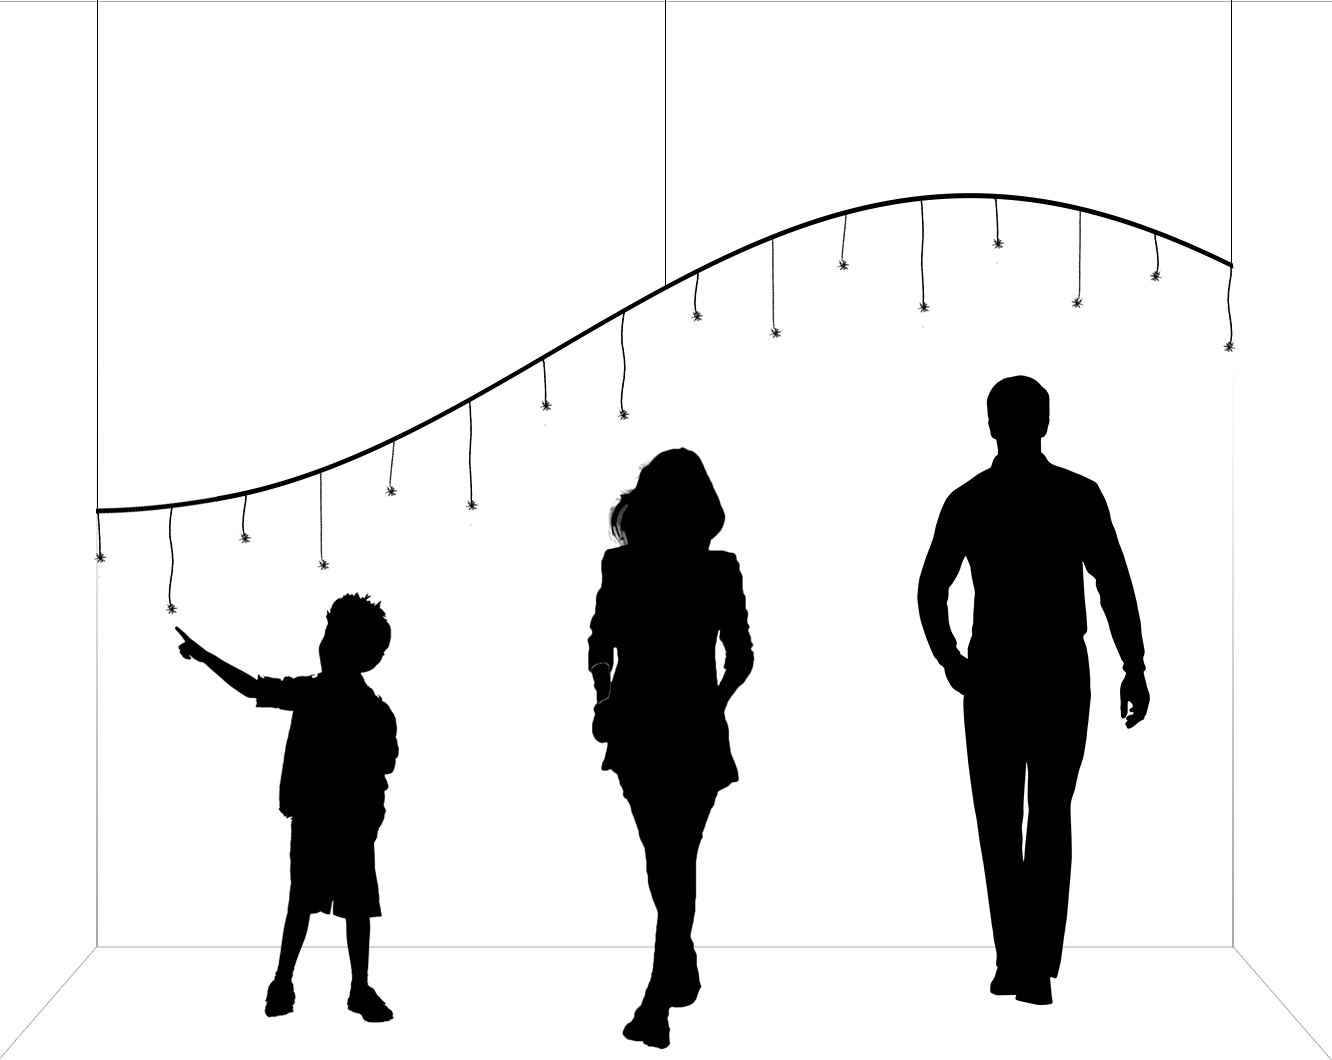
\includegraphics[width=0.8\textwidth]{./04-figuras/malha_futuro}
    \label{fig:malha_futuro}
\end{figure}
\vspace*{-0,9cm}
{\raggedright \fonte{Elaborada pela autora}}\\


Outro caminho natural de desenvolvimento diz respeito a aplicação e otimização de efeitos. Através de alteração do \textit{script} e utilização de portas analógicas seria possível controlar a intensidade do LED de acordo com a distância do espectador, fazendo-o acender ou apagar gradualmente à medida que o interator se afasta ou se aproxima. Além disso, também poderiam ser trabalhadas a manipulação de cores distintas através da utilização de LEDs RGB, neste caso, as possibilidades de variação dentro do mesmo trabalho são infinitas.

